% Formatiere den Text als Artikel mit KOMA-Script
% Schriftgröße ist 10 Punkt, zweispaltiges Layout
\documentclass[10pt,twocolumn,twoside,BCOR=10mm,DIV=calc,headings=small,parskip=half]{scrartcl}

% Normalerweise sollte man den Satzspiegel der Dokumentklasse überlassen. Bei
% zweispaltigem Layout ist mir aber der Randbereich zu groß
%\typearea{14}

% Englische und deutsche Übersetzungen von vordefinierten Bezeichnungen
\usepackage[english,german]{babel}

% Zeichensatz der Texte - Editor muss in UTF-8 kodiert speichern
\usepackage[utf8]{inputenc}

% erweiterte Befehle zur Formatierung von Formeln und mathematischem Inhalt 
\usepackage{amsmath}

% Befehle zum Einbinden von Grafiken und Bildern
\usepackage{graphicx}

%
%\usepackage{textcomp}

% zeigt Querverweise und Markierungen an
%\usepackage{showkeys}

% Provides commands for the geralpha.bst,...
%\usepackage{bibgerm}


\title{Formelsammlung Physik und Chemie}
\author{B. Süssmann,  J. Laumann}


% Provides hyperlinks and PDF output formatting
\usepackage[colorlinks=false,pdfborder={0 0 0}]{hyperref}
\makeatletter
\hypersetup{
 pdftitle={\@title},
 pdfsubject={},
 pdfkeywords={}
 pdfauthor={\@author},
}
\makeatother

  
% SI-Einheiten mit den Befehlen \SI und \si richtig formatieren
\usepackage{siunitx}
\sisetup{
 % SI-Einheiten werden mit Dezimal-PUNKT angegeben (könnte man ändern, gefällt
 % mir aber so besser, weil das Zusammenspiel mit CAS und anderen Programmen
 % besser funktioniert) - die Ausgabe erfolgt aber wie im deutschen Sprachraum
 % mit Dezimalkomma
 output-decimal-marker = {,},
 % in wissenschaftlicher Schreibweise soll zwischen Mantisse und Exponent ein
 % Multiplikationspunkt stehen
 exponent-product = \cdot,
 % Einheiten mit Brüchen sollen als Brüche dargestellt werden
 per-mode = fraction
}

\usepackage[version=3]{mhchem}

\usepackage[T1]{fontenc}
\usepackage{cmbright}

% XMP Metadaten einfügen
\usepackage{xmpincl}
\includexmp{metadata}

% Abstand zwischen den Spalten im mehrspaltigen Layout
\setlength{\columnsep}{1cm}

% Linie der Breite 0.5 Punkt zwischen den Spalten 
\setlength{\columnseprule}{0.5pt}

% In dieser Datei wird der Kopf und Fuß für die Formelsammlung definiert

\usepackage{fancyhdr}
\pagestyle{fancy}

\makeatletter

\fancypagestyle{firstpage}{\fancyhf{}%
\lhead{\includegraphics[height=1cm]{abslogo.png}}
  \chead{\sffamily\bfseries\@title}
\rhead{} 
\lfoot{
\includegraphics[height=0.7cm]{by-sa.png} \sffamily\tiny\@author}
\cfoot{}
\rfoot{\sffamily\tiny \selectlanguage{german}\@date}}

\lhead{}
\chead{\sffamily\bfseries\@title}
\rhead{} 
\fancyfoot{} % Fußzeile leeren
\fancyfoot[RE,LO]{\sffamily\tiny \selectlanguage{german}\@date}
\fancyfoot[RO,LE]{\sffamily Seite \thepage}
\makeatother 

\renewcommand{\headheight}{0.6in}
\renewcommand{\headrulewidth}{0.4pt}
%\renewcommand{\footrulewidth}{0.4pt}


% setze den Gleichungszähler mit jedem Abschnitt zurück
% -> Gleichungsnumerierung (Abschnitt.Gleichung)
\numberwithin{equation}{section}

% hier beginnt das eigentliche Dokument
\begin{document}
\thispagestyle{firstpage}

\section{Allgemeines}
\subsection{Konstanten}
% !TeX root=abs_formeln.tex

\begin{align}
\label{eq:konstanten:fallbeschleunigung}
g &= \SI{9.81}{\meter\per\second\squared}\\
\label{eq:konstanten:lichtgeschwindigkeit}
c &= \SI{3d8}{\meter\per\second}\\
\label{eq:konstanten:elementarladung}
e &= \SI{1.6021773d-19}{\coulomb}\\
\label{eq:konstanten:elektrische:feldkonstante}
\varepsilon_0 &= \SI{8.85d-12}{\coulomb\per\volt\per\meter}\\
\label{eq:konstanten:magnetische:feldkonstante}
\mu_0 &= \SI{1.257d-6}{\volt\second\per\ampere\per\meter}\\
\label{eq:konstanten:planck:konstante}
h &= \SI{6.626d-34}{\joule\second}\\
\label{eq:konstanten:atomare:masseneinheit}
u &= \SI{1.66054d-27}{\kilogram}\\
\label{eq:konstanten:avogadro:konstante}
N_A &= \SI{6.022d23}{\per\mol}\\
\label{eq:konstanten:masse:elektron}
m_e &= \SI{9.1d-31}{\kilogram}\\
\label{eq:konstanten:masse:neutron}
m_n &= \SI{1.675d-27}{\kilogram}\\
\label{eq:konstanten:masse:proton}
m_p &= \SI{1.673d-27}{\kilogram}\\
\label{eq:konstanten:allgemeine:gaskonstante}
R &= \SI{8.31}{\joule\per\mol\per\kelvin}
\end{align}
 
\subsection{Einheiten}
% !TeX root=abs_formeln.tex

\begin{align}
\label{eq:einheit:energie}
\left[P\right] &= \SI{1}{\watt} = \SI{1}{\joule\per\second} = \SI{1}{\volt\ampere}\\
\left[W\right] &= \SI{1}{\joule} = \SI{1}{\newton\meter} =
\SI{1}{\volt\ampere\second}\\
\label{eq:einheit:kraft}
\left[F\right] &= \SI{1}{\newton} = \SI{1}{\kilogram\meter\per\second\squared}\\
\label{eq:einheit:ladung}
\left[Q\right] &= \SI{1}{\coulomb} = \SI{1}{\ampere\second}\\
\label{eq:einheit:widerstand}
\left[R\right] &= \SI{1}{\ohm} = \SI{1}{\volt\per\ampere}\\
\label{eq:einheit:kapazitaet}
\left[C\right] &= \SI{1}{\farad} =
\SI{1}{\coulomb\per\volt}\\
\label{eq:einheit:magnetische:flussdichte}
\left[B\right] &= \SI{1}{\tesla} = \SI{1}{\newton\per\ampere\per\meter}\\
\label{eq:einheit:induktivitaet}
\left[L\right] &= \SI{1}{\henry} = \SI{1}{\volt\second\per\ampere}\\
\label{eq:einheit:elektrisches:feld}
\left[E\right] &= \SI{1}{\volt\per\meter} = \SI{1}{\newton\per\coulomb}\\
\label{eq:einheit:magnetischer:fluss}
\left[\Phi\right] &= \SI{1}{\tesla\meter\squared} = \SI{1}{\volt\second}\\
\label{eq:einheit:elektrische:flussdichte}
\left[\sigma\right] &= \SI{1}{\coulomb\per\meter\squared}\\
\label{eq:einheit:frequenz}
\left[f\right] &= \SI{1}{\per\second} = \SI{1}{\hertz}
\end{align}
 
\subsection{Einheitenpräfixe}
% !TeX root=abs_formeln.tex

\begin{small}
\begin{tabular}{|c|c|c|c|c|c|c|}
\hline
\si{\tera} & \si{\giga} & \si{\mega} & \si{\kilo} & \si{\hecto} & \si{\deca} & \\
\hline
\rule{0mm}{1em}$10^{12}$ & $10^{9}$ & $10^6$ & $10^3$ & $10^2$ & $10^1$ & $10^0$\\
\hline
\hline
  & \si{\deci} & \si{\centi} & \si{\milli} & \si{\micro} & \si{\nano} & \si{\pico}\\
\hline
\rule{0mm}{1em}$10^0$ & $10^{-1}$ & $10^{-2}$ & $10^{-3}$ & $10^{-6}$ & $10^{-9}$ &
$10^{-12}$\\
\hline
\end{tabular}
\end{small}
 
\subsection{Griechische Buchstaben}
% !TeX root=abs_formeln.tex

\begin{small}
\begin{tabular}{clclcl}
$\alpha$, $A$ & Alpha & $\beta$, $B$ & Beta & $\gamma$ , $\Gamma$ & Gamma \\
$\delta$, $\Delta$ & Delta & $\varepsilon$, $E$ & Epsilon & $\zeta$, $Z$ & Zeta\\
$\eta$, $H$ & Eta & $\vartheta$, $\Theta$ & Theta & $\iota$, $I$ & Iota \\
$\kappa$, $K$ & Kappa & $\lambda$, $L$ & Lambda & $\mu$, $M$ & My\\
$\nu$, $N$ & Ny & $\xi$, $\Xi$ & Xi & $o$, $O$ & Omikron \\
$\pi$, $\Pi$ & Pi & $\varrho$, $R$ & Rho & $\sigma$, $\Sigma$ & Sigma\\
$\tau$, $T$ & Tau & $\upsilon$, $Y$ & Ypsilon & $\varphi$, $\Phi$ & Phi\\
$\chi$, $X$ & Chi & $\psi$, $\Psi$ & Psi & $\omega$, $\Omega$ & Omega
\end{tabular}
\end{small}

\subsection{Mathematik}
% !TeX root=abs_formeln.tex

\subsubsection{Kugeloberfläche}
\begin{equation}\label{eq:mathematik:kreisflaeche}
 A = 4\cdot \pi \cdot r^2
\end{equation}

\subsubsection{Kugelvolumen}
\begin{equation}\label{eq:mathematik:kugelvolumen}
 V = \frac{4}{3}\cdot\pi\cdot r^3
\end{equation}

\subsubsection{pq-Formel}
\begin{equation}\label{eq:mathematik:quadratische:gleichung:pq}
x_{1,2} = - \frac{p}{2} \pm \sqrt{ \left(\frac{p}{2}\right)^2 - q }
\end{equation}
mit $ 0 = x^2 + p \cdot x + q $

\subsubsection{Trigonometrische Beziehungen}
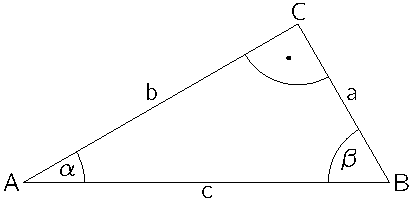
\includegraphics[width=0.6\linewidth]{trigonometrie} \hfill
%\begin{minipage}[b]{.55\linewidth}\raggedright
\begin{align}
\sin\alpha &= \frac{a}{c} = \frac{\text{Gegenkathete}}{\text{Hypotenuse}}\\
\cos\alpha &= \frac{b}{c} = \frac{\text{Ankathete}}{\text{Hypotenuse}}\\
\tan\alpha  &= \frac{a}{b} = \frac{\text{Gegenkathete}}{\text{Ankathete}}
\end{align}
%\end{minipage}

 
\section{Mechanik}
% !TeX root=abs_formeln.tex

\subsection{Geradlinige, gleichförmige Bewegung}
\begin{equation}\label{eq:mechanik:geradlinige:gleichfoermige:bewegung:v}
v = \frac{\Delta s}{\Delta t}
\end{equation}

\subsection{Geradlinige, gleichmäßig beschleunigte Bewegung}
\begin{equation}\label{eq:mechanik:geradlinige:gleichmaessig:beschleunigte:bewegung:a}
a = \frac{\Delta v}{\Delta t}
\end{equation}

\begin{equation}\label{eq:mechanik:geradlinige:gleichmaessig:beschleunigte:bewegung:s:v}
\Delta s = \frac{(v_2 + v_1) \cdot \Delta t}{2}
\end{equation}  

\begin{equation}\label{eq:mechanik:geradlinige:gleichmaessig:beschleunigte:bewegung:s:a}
s(t) = \frac{1}{2}\cdot a\cdot t^2 + v_0 \cdot t + s_0
\end{equation}

\subsection{Grundgleichung der Mechanik (Newtons Grundgesetz)}
\begin{equation}\label{eq:mechanik:grundgleichung}
 F = m \cdot a
\end{equation}

\subsection{Gewichtskraft}
\begin{equation}\label{eq:mechanik:gewichtskraft}
 F_G = m \cdot g
\end{equation}

\subsection{Hookesches Gesetz}
\begin{equation}\label{eq:mechanik:hookesches:gesetz}
 F = D \cdot s
\end{equation}

\subsection{Schiefe Ebene}
\begin{equation}\label{eq:mechanik:schiefe:ebene:hangabtriebskraft}
 F_H = F_G \cdot \sin \alpha
\end{equation}

\begin{equation}\label{eq:mechanik:schiefe:ebene:normalkraft}
 F_N = F_G \cdot \cos \alpha
\end{equation}

\subsection{Reibung}
\begin{equation}\label{eq:mechanik:reibung:ordnung}
 F_h > F_{gl} > F_{roll}
\end{equation}

\begin{equation}\label{eq:mechanik:gleitreibung:kraft}
 F_{gl} = f_{gl} \cdot F_N 
\end{equation}

\begin{equation}\label{eq:mechanik:haftreibung:maximale:kraft}
 F_{h,max} = f_{h} \cdot F_N 
\end{equation}

\subsection{Bremsverzögerung}
\begin{equation}\label{eq:mechanik:gleitreibung:bremsverzoegerung}
 \left| a \right| = f_{gl} \cdot g
\end{equation}

\begin{equation}\label{eq:mechanik:haftreibung:bremsverzoegerung}
 \left| a \right| = f_{h} \cdot g
\end{equation}

\subsection{Zentripetalkraft}
\begin{equation}\label{eq:mechanik:zentripetalkraft}
 F_z = \frac{m \cdot v^2}{r}
\end{equation}

\subsection{Energieerhaltung}
\begin{align}
\label{eq:mechanik:energieerhaltung}
 W_L + W_B + W_{Sp}  &= \text{konst.}\\
\label{eq:mechanik:lageenergie}
 W_L  &= m \cdot g \cdot h \\
\label{eq:mechanik:bewegungsenergie}
 W_B &= \frac{1}{2}\cdot m \cdot v^2 \\
\label{eq:mechanik:spannenergie}
W_{Sp} &=  \frac{1}{2} \cdot D \cdot s^2
\end{align}

\subsection{Energie / Arbeit}
\begin{equation}\label{eq:mechanik:energie}
 W = F_s \cdot s
\end{equation}

\subsection{Leistung}
\begin{equation}\label{eq:mechanik:leistung}
 P = \frac{\Delta W}{\Delta t}
\end{equation}

\subsection{Impuls}
\begin{equation}\label{eq:mechanik:impuls}
 p = m \cdot v
\end{equation}

\subsection{Impulserhaltung}
\begin{equation}\label{eq:mechanik:impulserhaltung}
 m_1 \cdot u_1 + m_2 \cdot u_2 = m_1 \cdot v_1 + m_2 \cdot v_2 
\end{equation}
 
\section{Elektrische und magnetische Felder}
% !TeX root=abs_formeln.tex

\subsection{Stromstärke}
\begin{equation}\label{eq:elektrischer:strom}
I = \frac{\Delta Q}{\Delta t}
\end{equation}

\begin{equation}\label{eq:elektrischer:strom:elektronen}
I = \frac{n \cdot e \cdot v}{\Delta s}
\end{equation}

\subsection{Elektrische Feldstärke}
\begin{equation}\label{eq:elektrische:feldstaerke}
E = \frac{F}{q}
\end{equation}

\subsection{Bifilares Plättchen im elektrischen Feld}
\begin{equation}\label{eq:bifilares:plaettchen:1}
F = F_G \cdot \frac{s}{h}
\end{equation}

\begin{equation}\label{eq:bifilares:plaettchen:2}
F \approx F_G \cdot \frac{s}{\ell}
\end{equation}

\subsection{Elektrische Spannung}
\begin{equation}\label{eq:elektrische:spannung}
U = \frac{W}{q}
\end{equation}

\begin{equation}\label{eq:elektrische:spannung:feld}
U = E \cdot d
\end{equation}

\subsection{Ohmsches Gesetz}
\begin{equation}\label{eq:ohmsches:gesetz}
U = R \cdot I
\end{equation}

\subsection{Spezifischer Widerstand}
\begin{equation}\label{eq:spezifischer:widerstand}
R = \varrho\cdot\frac{\ell}{A}
\end{equation}

\subsection{Elektrische Energie}
\begin{equation}\label{eq:elektrische:energie}
W = U \cdot I \cdot t
\end{equation}

\subsection{Elektrische Leistung}
\begin{equation}\label{eq:elektrische:leistung}
P = \frac{W}{t} = U \cdot I
\end{equation}

\subsection{Reihenschaltung von Widerständen}
\begin{equation}\label{eq:widerstand:reihenschaltung:spannung}
U = U_1 + U_2 
\end{equation}

\begin{equation}\label{eq:widerstand:reihenschaltung:strom}
I = I_1 = I_2
\end{equation}

\begin{equation}\label{eq:widerstand:reihenschaltung:widerstand}
R = R_1 + R_2
\end{equation}

\subsection{Parallelschaltung von Widerständen}
\begin{equation}\label{eq:widerstand:parallelschaltung:spannung}
U = U_1 = U_2
\end{equation}

\begin{equation}\label{eq:widerstand:parallelschaltung:strom}
I = I_1 + I_2
\end{equation}

\begin{equation}\label{eq:widerstand:parallelschaltung:widerstand}
\frac{1}{R} = \frac{1}{R_1} + \frac{1}{R_2} 
\end{equation}

\subsection{Elektrisches Potential}
\begin{equation}\label{eq:elektrisches:potential}
\Delta \varphi = \varphi_2 - \varphi_1
\end{equation}

\subsection{Flächenladungsdichte}
\begin{equation}\label{eq:flaechenladungsdichte}
\sigma = \frac{Q}{A}
\end{equation}

\begin{equation}\label{eq:flaechenladungsdichte:feld}
\sigma = \varepsilon_0 \cdot \varepsilon_r \cdot E
\end{equation}

\subsection{Coulomb-Gesetz}
\begin{equation}\label{eq:coulomb:gesetz}
F = q \cdot E = \frac{1}{4\cdot \pi \cdot \varepsilon_0}\cdot \frac{Q \cdot
 q}{r^2}
\end{equation}

\subsection{Coulomb-Potential}
\begin{equation}\label{eq:coulomb:potential}
\varphi = \frac{1}{4\cdot \pi \cdot \varepsilon_0}\cdot \frac{Q}{r}
\end{equation}

\begin{equation}\label{eq:coulomb:potential:energie}
W_{12} = \frac{Q \cdot q}{4\cdot \pi \cdot
 \varepsilon_0}\cdot\left(\frac{1}{r_1} - \frac{1}{r_2}\right)
\end{equation}

\begin{equation}\label{eq:coulomb:potential:spannung}
U_{12} = \frac{Q}{4\cdot \pi \cdot
 \varepsilon_0}\cdot\left(\frac{1}{r_1} - \frac{1}{r_2}\right)
\end{equation}

\subsection{Kondensatoren}
\begin{equation}\label{eq:kondensator:kapazitaet}
C = \frac{Q}{U}
\end{equation}

\begin{equation}\label{eq:kondensator:kapazitaet:platten}
C = \varepsilon_0 \cdot \varepsilon_r \cdot \frac{A}{d}
\end{equation}

\subsection{Kugelkondensator}
\begin{equation}\label{eq:kondensator:kapazitaet:kugel}
C = \frac{4\cdot\pi\cdot\varepsilon_0}{\frac{1}{r_1}-\frac{1}{r_2}}
\end{equation}

\subsection{Reihenschaltung von Kondensatoren}
\begin{equation}\label{eq:kondensator:reihenschaltung:ladung}
Q = Q_1 = Q_2
\end{equation}
 
\begin{equation}\label{eq:kondensator:reihenschaltung:spannung}
U = U_1 + U_2 
\end{equation}
 
\begin{equation}\label{eq:kondensator:reihenschaltung:kapazitaet}
\frac{1}{C} = \frac{1}{C_1} + \frac{1}{C_2}
\end{equation}

\subsection{Parallelschaltung von Kondensatoren}
\begin{equation}\label{eq:kondensator:parallelschaltung:ladung}
Q = Q_1 + Q_2
\end{equation}

\begin{equation}\label{eq:kondensator:parallelschaltung:spannung}
U = U_1 = U_2
\end{equation}

\begin{equation}\label{eq:kondensator:parallelschaltung:kapazitaet}
C = C_1 + C_2
\end{equation}

\subsection{Kondensatorentladung}
\begin{equation}\label{eq:kondensator:entladung:zeit}
T_H = \SI{0.69}{} \cdot R \cdot C
\end{equation}

\begin{equation}\label{eq:kondensator:entladung:spannung}
U(t) = U_0 \cdot 2^{-\frac{t}{T_H}}
\end{equation}

\begin{equation}\label{eq:kondensator:entladung:ladung}
Q(t) = Q_0 \cdot 2^{-\frac{t}{T_H}}
\end{equation}

\begin{equation}\label{eq:kondensator:entladung:strom}
I(t) = I_0 \cdot 2^{-\frac{t}{T_H}}
\end{equation}

\subsection{Energie eines geladenen Kondensators}
\begin{equation}\label{eq:kondensator:energie:spannung}
W = \frac{1}{2} \cdot C \cdot U^2
\end{equation}

\begin{equation}\label{eq:kondensator:energie:feld}
W = \frac{1}{2} \cdot \varepsilon_0 \cdot \varepsilon_r \cdot E^2 \cdot V
\end{equation}

\subsection{Räumliche Dichte der elektrischen Energie}
\begin{equation}\label{eq:rauemliche:dicht:elektrische:energie}
\varrho_{el} = \frac{W}{V} = \frac{1}{2} \cdot \varepsilon_0 \cdot \varepsilon_r \cdot
 E^2
\end{equation}

\subsection{Anziehungskraft zwischen zwei Kondensatorplatten}
\begin{equation}\label{eq:kondensator:anziehungskraft}
F = \frac{\Delta W}{\Delta s}
\end{equation}

\begin{equation}\label{eq:kondensator:anziehungskraft:elektrisches:feld}
F = \frac{1}{2}\cdot\varepsilon_0 \cdot
\varepsilon_r \cdot E^2 \cdot A
\end{equation}

\begin{equation}\label{eq:kondensator:anziehungskraft:spannung}
F = \frac{1}{2}\cdot\varepsilon_0 \cdot \varepsilon_r \cdot
 \frac{U^2}{d^2} \cdot A
\end{equation}

\subsection{Magnetische Flussdichte}
\begin{equation}\label{eq:magnetische:flussdichte}
B = \frac{F}{I \cdot s}
\end{equation}

\begin{equation}\label{eq:magnetische:flussdichte:schlanke:spule}
B = \mu_0 \cdot \mu_r \cdot \frac{n}{\ell} \cdot I
\end{equation}

\begin{equation}\label{eq:magnetische:flussdichte:relative:permeabilitaet}
\mu_r = \frac{B_m}{B_0}
\end{equation}

\subsection{Lorentzkraft}
\begin{equation}\label{eq:lorentzkraft}
F_L = Q \cdot v_s \cdot B
\end{equation}

\subsection{Hall-Spannung}
\begin{equation}\label{eq:hall:spannung}
U_H = B \cdot v_s \cdot h
\end{equation}

\subsection{Magnetfeld der Erde}
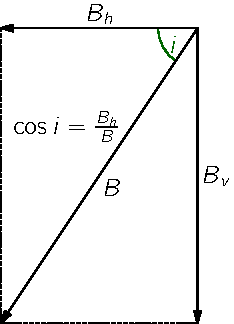
\includegraphics[width=.4\linewidth]{magnetfeld_der_erde} \hfill
\begin{minipage}[b]{.55\linewidth}\raggedright
Inklinationswinkel: $i$

Horizontalkomponente des Erdmagnetfelds: $B_h$

Vertikalkomponente des Erdmagnetfelds: $B_v$
\end{minipage}

\subsection{Ladungen im Magnetfeld}
\begin{equation}\label{eq:magnetfeld:elektronen:kreisbahn}
r = \frac{v_s \cdot m}{B \cdot q}
\end{equation}

\subsection{Magnetische Induktion}
Anzahl der Leiterschleifen: $n$

$A_s$ ist die senkrecht von den Feldlinien durchsetzte Fläche. Sie ist mit Hilfe der trigonometrischen Funktionen aus A berechenbar.
 
\subsubsection{durch Leiterbewegung}
\begin{equation}\label{eq:magnetische:induktion:leiterbewegung}
U_{ind} = n \cdot B \cdot d \cdot v_s
\end{equation}

\subsubsection{durch Flächenänderung}
\begin{equation}\label{eq:magnetische:induktion:flaechenaenderung}
U_{ind} = n \cdot B \cdot d \cdot v_s = n \cdot B \cdot \frac{\Delta A_s}{\Delta t}
\end{equation}

\subsubsection{durch Drehung}
\begin{equation}\label{eq:magnetische:induktion:drehung}
U_{ind} = n \cdot B \cdot \frac{\Delta A_s}{\Delta t}
\end{equation}

\subsubsection{durch Flussdichteänderung}
\begin{equation}\label{eq:magnetische:induktion:flussdichteaenderung}
U_{ind} = n \cdot A_s \cdot \frac{\Delta B}{\Delta t}
\end{equation}
  
\subsubsection{durch Änderung des magnetischen Flusses}
\begin{equation}\label{eq:magnetische:induktion:flussaenderung}
U_{ind}(t) = n \cdot \frac{\Delta \Phi}{\Delta t}
\end{equation}

\subsubsection{Momentanspannung für $\Delta t \to 0$}
\begin{equation}\label{eq:magnetische:induktion:momentanspannung}
U_{ind}(t) = n \cdot \dot{\Phi}(t)
\end{equation}

\subsection{Magnetischer Fluss}
\begin{equation}\label{eq:magnetischer:fluss}
\Phi = B \cdot A_s
\end{equation}

\subsection{Selbstinduktion einer Spule}
\begin{equation}\label{eq:spule:selbstinduktion}
U_{ind}(t) = - n \cdot \dot{\Phi}(t) = - L \cdot \dot{I}(t)
\end{equation}
\begin{equation}\label{eq:spule:induktivitaet}
L = \mu_0\cdot
\mu_r \cdot n^2 \cdot \frac{A}{\ell}
\end{equation}
 
\section{Schwingungen und Wellen}
% !TeX root=abs_formeln.tex

\begin{equation}\label{eq:schwingung:frequenz}
f = \frac{n}{t} = \frac{1}{T}
\end{equation}

\subsection{Harmonische Schwingung}
$\varphi = \text{Phasenwinkel}$, $\SI{360}{\degree} \hat{=} 2\pi $

\subsubsection{Winkelgeschwindigkeit $\omega$}
\begin{equation}\label{eq:schwingung:winkelgeschwindigkeit}
\omega = \frac{\varphi}{t} = \frac{2 \pi}{T} = 2 \pi f
\end{equation}

\subsubsection{Elongation $s$}
\begin{equation}\label{eq:schwingung:elongation}
s = r \cdot \sin \varphi \quad \hat{s} = r
\end{equation}

\subsubsection{Zeit-Weg-Gesetz}
\begin{equation}\label{eq:schwingung:t:s:gesetz}
s(t) = \hat{s}\cdot\sin(\omega\cdot t)
\end{equation}

\subsubsection{Zeit-Geschwindigkeits-Gesetz}
\begin{equation}\label{eq:schwingung:t:v:gesetz}
v(t) = \omega \cdot \hat{s} \cdot \cos(\omega \cdot t)
\end{equation}

\subsubsection{Zeit-Beschleunigungs-Gesetz}
\begin{equation}\label{eq:schwingung:t:a:gesetz}
a(t) = - \omega^2 \cdot \hat{s} \cdot \sin(\omega \cdot t)
\end{equation}

\begin{equation}\label{eq:schwingung:beschleunigung:allgemein}
a(t) = \dot{v}(t) = \ddot{s}(t)
\end{equation}

\subsubsection{Elongations-Kraft-Gesetz}
(Bedingung für harmonische Schwingung)
\begin{equation}\label{eq:schwingung:ruecktreibende:kraft}
F = - D \cdot s
\end{equation}
mit Richtgröße $D$
\begin{equation}\label{eq:schwingung:richtgroesse}
D = m \cdot \omega^2
\end{equation}
liefert die Periodendauer
\begin{equation}\label{eq:schwingung:periodendauer}
T = 2\pi \sqrt{\frac{m}{D}}
\end{equation}

\subsubsection{Energie einer ungedämpften harmonischen Schwingung}
\begin{equation}\label{eq:energie:ungedaempfte;harmonische:schwingung}
\begin{split}
W &= W_{Elong} + W_B \\
   &= \frac{1}{2} D \cdot s^2 + \frac{1}{2} m \cdot v^2 = \text{konst.}
\end{split}
\end{equation}

\subsubsection{Schwingung des Fadenpendels}
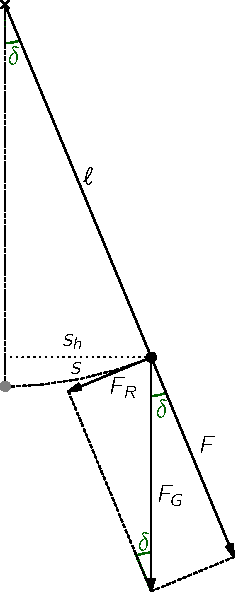
\includegraphics[width=.35\linewidth]{fadenpendel}
\hfill
\begin{minipage}[b]{.6\linewidth}
Auslenkung des Pendels: $s$ 
\begin{equation}\label{eq:fadenpendel:auslenkung}
s = \ell\cdot\delta
\end{equation}

\begin{equation}\label{eq:fadenpendel:winkel}
\sin\delta = \frac{s_h}{\ell} \approx \frac{s}{\ell} 
\end{equation}

\begin{equation}\label{eq:fadenpendel:winkel:kraefte}
\sin\delta = \frac{F_R}{F_G}
\end{equation}

\begin{equation}\label{eq:fadenpendel:ruecktreibende:kraft}
F_R = \frac{m \cdot g \cdot s}{\ell}
\end{equation}

\begin{equation}\label{eq:fadenpendel:richtgroesse}
D = \frac{m \cdot g}{\ell}
\end{equation}

\begin{equation}\label{eq:fadenpendel:periodendauer}
T = 2 \pi\sqrt{\frac{\ell}{g}}
\end{equation}
\end{minipage}

\subsubsection{Elektromagnetischer Schwingkreis}
\begin{equation}\label{eq:elektromagnetischer:schwingkreis:ladung}
Q = \hat{Q}\cos(\omega \cdot t)\\
\end{equation}

\begin{equation}\label{eq:elektromagnetischer:schwingkreis:spannung}
U = \hat{U}\cos(\omega \cdot t)\\
\end{equation}

\begin{equation}\label{eq:elektromagnetischer:schwingkreis:stromstaerke}
I = - \hat{I}\sin(\omega \cdot t)
\end{equation}

\begin{equation}\label{eq:elektromagnetischer:schwingkreis:winkelgeschwindigkeit}
\omega = \frac{1}{\sqrt{L \cdot C}}
\end{equation}

\begin{equation}\label{eq:elektromagnetischer:schwingkreis:maximale:stromstaerke}
\hat{I} = \frac{\hat{U} \cdot C}{\sqrt{L \cdot C}}
\end{equation}

\begin{equation}\label{eq:elektromagnetischer:schwingkreis:periodendauer}
T = 2\pi \sqrt{L \cdot C}
\end{equation}

\subsubsection{Resonanzbedingung}
\begin{equation}\label{eq:resonanzbedingung}
f = f_0 \quad\text{mit}\quad \varphi = \frac{\pi}{2}
\end{equation}

\subsubsection{Eigenschwingungen zwischen zwei festen Enden}
\begin{equation}\label{eq:eigenschwingung:laengen}
\ell = k \cdot \frac{\lambda_k}{2} \quad k = 1, 2, 3,\ldots
\end{equation}

\begin{equation}\label{eq:eigenschwingung:frequenzen}
f_k = k \cdot \frac{c}{2 \cdot \ell} \quad k = 1, 2, 3,\ldots
\end{equation}
% !TeX root=abs_formeln.tex

\subsection{Ausbreitungsgeschwindigkeit}
\begin{equation}\label{eq:wellen:ausbreitungsgeschwindigkeit}
c = \frac{\lambda}{T} =
\frac{\Delta x}{\Delta t}
\end{equation}

\subsection{Wellengleichung}
\begin{eqnarray}\label{eq:wellen:gleichung}
s(t,x) &=& \hat{s} \cdot \sin \left[ \omega \left( t - \frac{x}{c} \right)
\right]\\
s(t,x) &=& \hat{s} \cdot \sin \left[ 2\pi \left( \frac{t}{T} - \frac{x}{\lambda}
\right) \right]
\end{eqnarray}

\subsection{Überlagerung von Schwingungen}
\begin{equation}
\begin{split}
\label{eq:schwingung:ueberlagerung}
s(t) &= s_1(t) + s_2(t) \\
&= \hat{s}_1 \cdot \sin(\omega \cdot t) + \hat{s}_2 \cdot
\sin(\omega \cdot t + \varphi_0)
\end{split}
\end{equation}

\subsection{Konstruktive Interferenz}
\begin{equation}
\begin{split}
\label{eq:konstruktive:interferenz}
\Delta \varphi &= 0, 2\pi, 4\pi,\dots\\
 \delta &= k \cdot \lambda, \quad k = 0, 1, 2, \ldots
\end{split}
\end{equation}

\subsection{Destruktive Interferenz}
\begin{equation}
\begin{split}
\label{eq:destruktive:interferenz}
\Delta \varphi &= \pi, 3\pi, 5\pi,\dots \\
 \delta &= (2\cdot k - 1) \cdot \frac{\lambda}{2}, \quad k = 1, 2, 3, \ldots
\end{split}
\end{equation}

\subsection{Verhältnis Gangunterschied zu Phasendifferenz}
\begin{equation}\label{eq:gangunterschied:phasendifferenz}
\frac{\Delta\varphi}{2\pi} = \frac{\delta}{\lambda}
\end{equation}

\subsection{Doppler-Effekt}
\subsubsection{Bewegter Beobachter, ruhender Sender}
\paragraph{Annähern}
\begin{equation}\label{eq:doppler:effekt:bewegter:beobachter:annaehern}
f' = f\cdot\left(1 + \frac{v}{c} \right)
\end{equation}

\paragraph{Entfernen}
\begin{equation}\label{eq:doppler:effekt:bewegter:beobachter:entfernen}
f' = f\cdot\left(1 - \frac{v}{c} \right)
\end{equation}

\subsubsection{Bewegter Sender, ruhender Beobachter}
\paragraph{Annähern}
\begin{equation}\label{eq:doppler:effekt:bewegter:sender:annaehern}
\lambda' = \lambda \cdot\left(1 - \frac{v_s}{c} \right) \quad
f' = \frac{f}{1 - \frac{v_s}{c}}
\end{equation}

\paragraph{Entfernen}
\begin{equation}\label{eq:doppler:effekt:bewegter:sender:entfernen}
f' = \frac{f}{1 + \frac{v_s}{c}}
\end{equation}

\subsubsection{Machsche Zahl}
\begin{equation}\label{eq:machsche:zahl}
M = \frac{v_s}{c}
\end{equation}

\subsection{Brechungsgesetz}
\begin{equation}\label{eq:brechungsgestz}
\frac{\sin\alpha}{\sin\beta} = \frac{c_1}{c_2}
\end{equation}

\subsection{Beugung und Interferenz am Doppelspalt}
\begin{center}
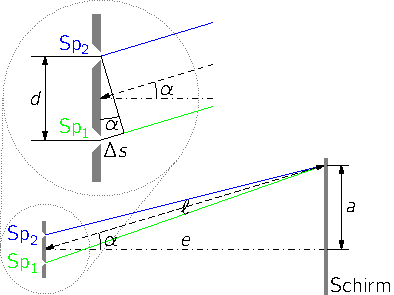
\includegraphics{doppelspalt}
\end{center}
\begin{equation}\label{eq:beugung:doppelspalt}
\sin\alpha = \frac{a}{\ell} = \frac{a}{\sqrt{e^2 + a^2}}
\end{equation}

\subsubsection{Maxima}
\begin{equation}\label{eq:interferenz:doppelspalt:maxima}
n\cdot \lambda = d \cdot \sin \alpha_n
\end{equation}

\subsubsection{Minima}
\begin{equation}\label{eq:interferenz:doppelspalt:minima}
(2\cdot n - 1) \cdot \frac{\lambda}{2} = d \cdot \sin \alpha_n
\end{equation}

\subsection{Beugung und Interferenz am Gitter}
\begin{equation}\label{eq:beugung:gitter}
n \cdot \lambda = g \cdot \sin\alpha_n = \frac{g \cdot a_n}{\ell} =
\frac{g \cdot a_n}{\sqrt{e^2 + a_n^2}}
\end{equation}

 
\section{Quantenphysik}
% !TeX root=abs_formeln.tex

\subsection{Photoeffekt}

\subsubsection{Maximale Energie der Photoelektronen}
\begin{equation}\label{eq:photoeffekt:maximale:energie:elektron}
W_{max} = e \cdot U_{max} \quad W_{max} = h \cdot f - W_A
\end{equation}

\subsubsection{Grenzfrequenz der Elektronenablösung}
\begin{equation}\label{eq:photoeffekt:grenzfrequenz}
f_{gr} = \frac{W_A}{h}
\end{equation}

\subsubsection{Photostrom}
\begin{equation}\label{eq:photoeffekt:photostrom}
I_{Ph} = Z \cdot \frac{e}{t}
\end{equation}

\subsection{Umkehrung des Photoeffekts}
\begin{equation}\label{eq:umgekehrter:photoeffekt:energie}
W_{El} = e \cdot U = h \cdot f
\end{equation}

\begin{equation}\label{eq:umgekehrter:photoeffekt:maximale:frequenz}
f_{max} = \frac{c}{\lambda_{min}}
\end{equation}

\begin{equation}\label{eq:umgekehrter:photoeffekt:energiebilanz}
h \cdot f_{max} = e \cdot U
\end{equation}

\subsection{Masse-Energie-Äquivalent}
\begin{equation}\label{eq:masse:energie:aequivalent}
W_0 = m_0 \cdot c^2
\end{equation}

\subsection{Masse der Photonen}
\begin{equation}\label{eq:photon:masse}
m = \frac{W}{c^2} = \frac{h \cdot f}{c^2}
\end{equation}

\subsection{Impuls der Photonen}
\begin{equation}\label{eq:photon:impuls}
p = m \cdot v = \frac{h \cdot f}{c} = \frac{h}{\lambda}
\end{equation}

\subsection{Paarbildung}
Photon $\rightarrow$ Elektron + Positron

\subsubsection{Energieerhaltung}
\begin{equation}\label{eq:paarbildung:energieerhaltung}
h \cdot f = 2\cdot m_e \cdot c^2 + 2 \cdot W_{kin} \ge
\SI{1.02}{\mega\electronvolt}
\end{equation}

\subsubsection{Massenerhaltung}
\begin{equation}\label{eq:paarbildung:massenerhaltung}
\frac{h\cdot f}{c^2} = \frac{2 \cdot W_{kin}}{c^2} + 2 \cdot m_e
\end{equation}

\subsubsection{Impulserhaltung}
\begin{equation}\label{eq:paarbildung:impulserhaltung}
\frac{h \cdot f}{c} = 2 \cdot m_e \cdot v < 2 \cdot m_e \cdot c \le
\frac{h \cdot f}{c}
\end{equation}

\subsection{Zerstrahlung}
Elektron + Positron $\rightarrow$ 2 Photonen

\subsubsection{Energieerhaltung}
\begin{equation}\label{eq:zerstrahlung:energieerhaltung}
2\cdot m_e \cdot c^2 = 2 \cdot h \cdot f =
\SI{1.02}{\mega\electronvolt}
\end{equation}

\subsubsection{Massenerhaltung}
\begin{equation}\label{eq:zerstrahlung:massenerhaltung}
2 \cdot m_e = \frac{2 \cdot h\cdot f}{c^2}
\end{equation}

\subsubsection{Impulserhaltung}
\begin{equation}\label{eq:zerstrahlung:impulserhaltung}
0 = \frac{h \cdot f}{c} + \left( - \frac{h \cdot f}{c} \right) 
\end{equation}

\subsection{Compton-Effekt}
\begin{equation}\label{eq:compton:effekt}
\Delta \lambda = \lambda' - \lambda = \lambda_C \cdot \left(1 - \cos\beta
\right)
\end{equation}

\begin{equation}\label{eq:compton:wellenlaenge}
\lambda_C = \frac{h}{m_e \cdot c} = \SI{2.4}{\pico\meter}
\end{equation}

\subsection{Photon als Quantenobjekt}
\begin{equation}\label{eq:photonquantenobjekt}
\Psi_{Res} = \Psi_1 + \Psi_2 \quad \left|\Psi_{Res}\right|^2 = \left|\Psi_1 +
\Psi_2\right|
\end{equation}
Antreffwahrscheinlichkeit: $\left|\Psi\right|^2$

 
\section{Kernphysik}
% !TeX root=abs_formeln.tex

\subsection{Abschätunzung der Kerngröße (Rutherford)}
\begin{equation}\label{eq:kerngroesse:rutherford}
\frac{1}{2}\cdot m\cdot v^2 = \frac{1}{4\cdot \pi \cdot \varepsilon_0}\cdot\frac{Z\cdot e\cdot 2\cdot e}{b}
\end{equation}

\subsection{Energie der Elektronen in der Atomhülle}
\begin{equation}\label{eq:potentielle:energie:elektron:atomhuelle}
W_p = - \frac{1}{4\cdot\pi\cdot\varepsilon_0}\cdot \frac{\left(Z\cdot e\right)\cdot e}{r}
\end{equation}

\begin{equation}\label{eq:kinetische:energie:elektron:atomhuelle}
W_k = \frac{1}{8\cdot\pi\cdot\varepsilon_0}\cdot \frac{\left(Z\cdot e\right)\cdot e}{r}
\end{equation}

\begin{equation}\label{eq:gesamt:energie:elektron:atomhuelle}
W_{ges} = - \frac{1}{8\cdot\pi\cdot\varepsilon_0}\cdot \frac{\left(Z\cdot e\right)\cdot e}{r}
\end{equation}

\subsection{Erstes Bohr-Postulat (Bahndrehimpuls)}
\begin{equation}\label{eq:erstes:bohr:postulat:1}
L = r \cdot m \cdot v = n \cdot \frac{h}{2\cdot\pi} \quad n = 1, 2, 3, \ldots
\end{equation}

\subsection{Zweites Bohr-Postulat (Frequenzbedingung)}
\begin{equation}\label{eq:zweites:bohr-postulat}
h\cdot f = E_m - E_n = \Delta E
\end{equation}

\subsection{Frequenz des Photons}
\begin{equation}\label{eq:bohr:frequenz:photon}
\begin{split}
f &= R \left(\frac{1}{n^2}-\frac{1}{m^2}\right)
\end{split}
\end{equation}

\subsubsection{Rydberg-Frequenz}
\begin{equation}\label{eq:rydberg:frequenz}
R = \frac{m_e \cdot e^4}{8 \cdot \varepsilon_0^2 \cdot h^3} = \SI{3.2898e15}{\hertz} 
\end{equation}

\subsection{Zerfallsgesetz}
\begin{equation}\label{eq:zerfallsgesetz:zerfallskonstante}
N(t) = N_0 \cdot e^{-\lambda \cdot t}
\end{equation}

\begin{equation}\label{eq:zerfallsgesetz:halbwertszeit}
N(t) = N_0 \cdot 2^{-\frac{t}{T_{1/2}}}
\end{equation}

\subsection{Zerfallskonstante}
\begin{equation}\label{eq:zerfallskonstante}
\lambda = \frac{\ln 2}{T_{1/2}}
\end{equation}

\subsection{Aktivität}
\begin{align}
\label{eq:aktivitaet}
A &= \frac{\Delta N}{\Delta t} \\
\label{eq:aktivitaet:t}
A(t) &= \lambda \cdot N(t) = A_0 \cdot
e^{-\lambda \cdot t}
\end{align}


\section{Chemie}
% !TeX root=abs_formeln.tex

\subsection{Stoffmengenberechnung}

\begin{align}\label{eq:chemie:stoffmengenberechnung}
n &= \frac{m}{M}\\
n &= \frac{V}{V_m}\\
n &= c\cdot V\\
\frac{n_1}{n_2} &= \frac{N_1}{N_2}
\end{align}

\subsection{Teilchenzahl}
\begin{equation}\label{eq:chemie:teilchenzahl}
N = n \cdot N_A
\end{equation}

\subsection{Massenanteil}
\begin{equation}
w = \frac{m}{m_L}
\end{equation}

\subsection{Massenwirkungsgesetz}
Für die Reaktion $\ce{\nu_A A + \nu_B B <=> \nu_c C + \nu_D D}$

\begin{equation}
K_C =\frac{c^{\nu_C}(C)\cdot c^{\nu_D}(D)}{c^{\nu_A}(A)\cdot c^{\nu_B}(B)}
\end{equation}

\begin{equation}
K_P =\frac{p^{\nu_C}(C)\cdot p^{\nu_D}(D)}{p^{\nu_A}(A)\cdot p^{\nu_B}(B)}
\end{equation}

\begin{equation}
\begin{split}
&K_P = K_C\cdot \left(R \cdot T\right)^{\Delta \nu} \\
&\text{mit}\quad \Delta v = (\nu_C + \nu_D) - (\nu_A + \nu_B)
\end{split}
\end{equation}

\subsection{Allgemeines Gasgesetz}

\begin{equation}
\label{eq:chemie:allgemeines:gasgesetz}
n \cdot R \cdot T = p \cdot V
\end{equation}

\subsection{Gleichgewichtskonstante}

\begin{equation}\label{eq:chemie:gleichgewichtskonstante}
\ln K(T) = - \frac{1}{R \cdot T} \cdot \Delta_R G_m^0
\end{equation}

\subsection{Säuren und Basen}

\begin{align}
\label{eq:chemie:saeuren:basen}
K_W = c\left(\ce{H3O+}\right) \cdot c\left(\ce{OH-}\right) = \SI{e-14}{\mol\squared\per\litre\squared}\\
pK_w = -\lg\frac{k_w}{\si{\mol\squared\per\litre\squared}} = 14 = pH + pOH\\
pH = -\lg\frac{c\left(\ce{H3O+}\right)}{\si{\mol\per\litre}}\\
c\left(\ce{H3O+}\right) = 10^{-pH}\\
pOH = -\lg\frac{c\left(\ce{OH-}\right)}{\si{\mol\per\litre}}
\end{align}

\subsection{Säurekonstante}
Für die Reaktion $\ce{HA + H2O <=> H3O+ + A-}$

\begin{align}
K_S = \frac{c\left(\ce{H3O+}\right) \cdot c\left(\ce{A-}\right)}{c\left(\ce{HA}\right)}\\
pK_S = -\lg\frac{K_S}{\si{\mol\per\litre}}
\end{align}

\subsection{Basenkonstante}
Für die Reaktion $\ce{B + H2O <=> OH- + BH+}$

\begin{align}
K_B = \frac{c\left(\ce{OH-}\right) \cdot c\left(\ce{BH+}\right)}{c\left(\ce{B}\right)}\\
pK_B = -\lg\frac{K_B}{\si{\mol\per\litre}}\\
pK_B = 14 - pK_S
\end{align}

\subsection{Puffergleichung}

\begin{equation}
pH = pK_S + \lg\frac{c\left(\text{Base}\right)}{c\left(\text{Säure}\right)}
\end{equation}

\subsection{Löslichkeitsprodukt}

\begin{equation}
K_L\left(A_mB_n\right) = c^m\left(A\right) \cdot c^n\left(B\right)
\end{equation}

\subsection{Nernstsche Gleichung}

\begin{equation}
\begin{split}
U_H\left(Me^{z+} / Me\right) &= U_H^0\left(Me^{z+} / Me\right) \\
 &+ \frac{\SI{0.059}{\volt}}{z} \cdot \lg\frac{c\left(Me^{z+}\right)}{\si{\mol\per\litre}}
\end{split}
\end{equation}

\subsection{Reaktionsenthalpie}

\begin{align}
\Delta_R H &= - Q = -c_p \cdot m \cdot \Delta T\\
\Delta_R H_m^0 &= \sum\Delta_fH_m^0\left(\text{Produkte}\right) - \sum\Delta_fH_m^0\left(\text{Edukte}\right)
\end{align}

\subsection{Entropie}

\begin{equation}
\Delta_R S_m^0 = \sum S_m^0\left(\text{Produkte}\right) + \sum S_m^0\left(\text{Edukte}\right)
\end{equation}

\subsection{Freie Enthalpie und Gibbs-Helmholtzgleichung}

\begin{align}
\Delta_R G_m &= \Delta_R H_m - T \cdot \Delta_R S_m\\
\Delta_R G_m^0 &= \sum\Delta_fG_m^0\left(\text{Produkte}\right) - \sum\Delta_fG_m^0\left(\text{Edukte}\right)
\end{align}



\onecolumn
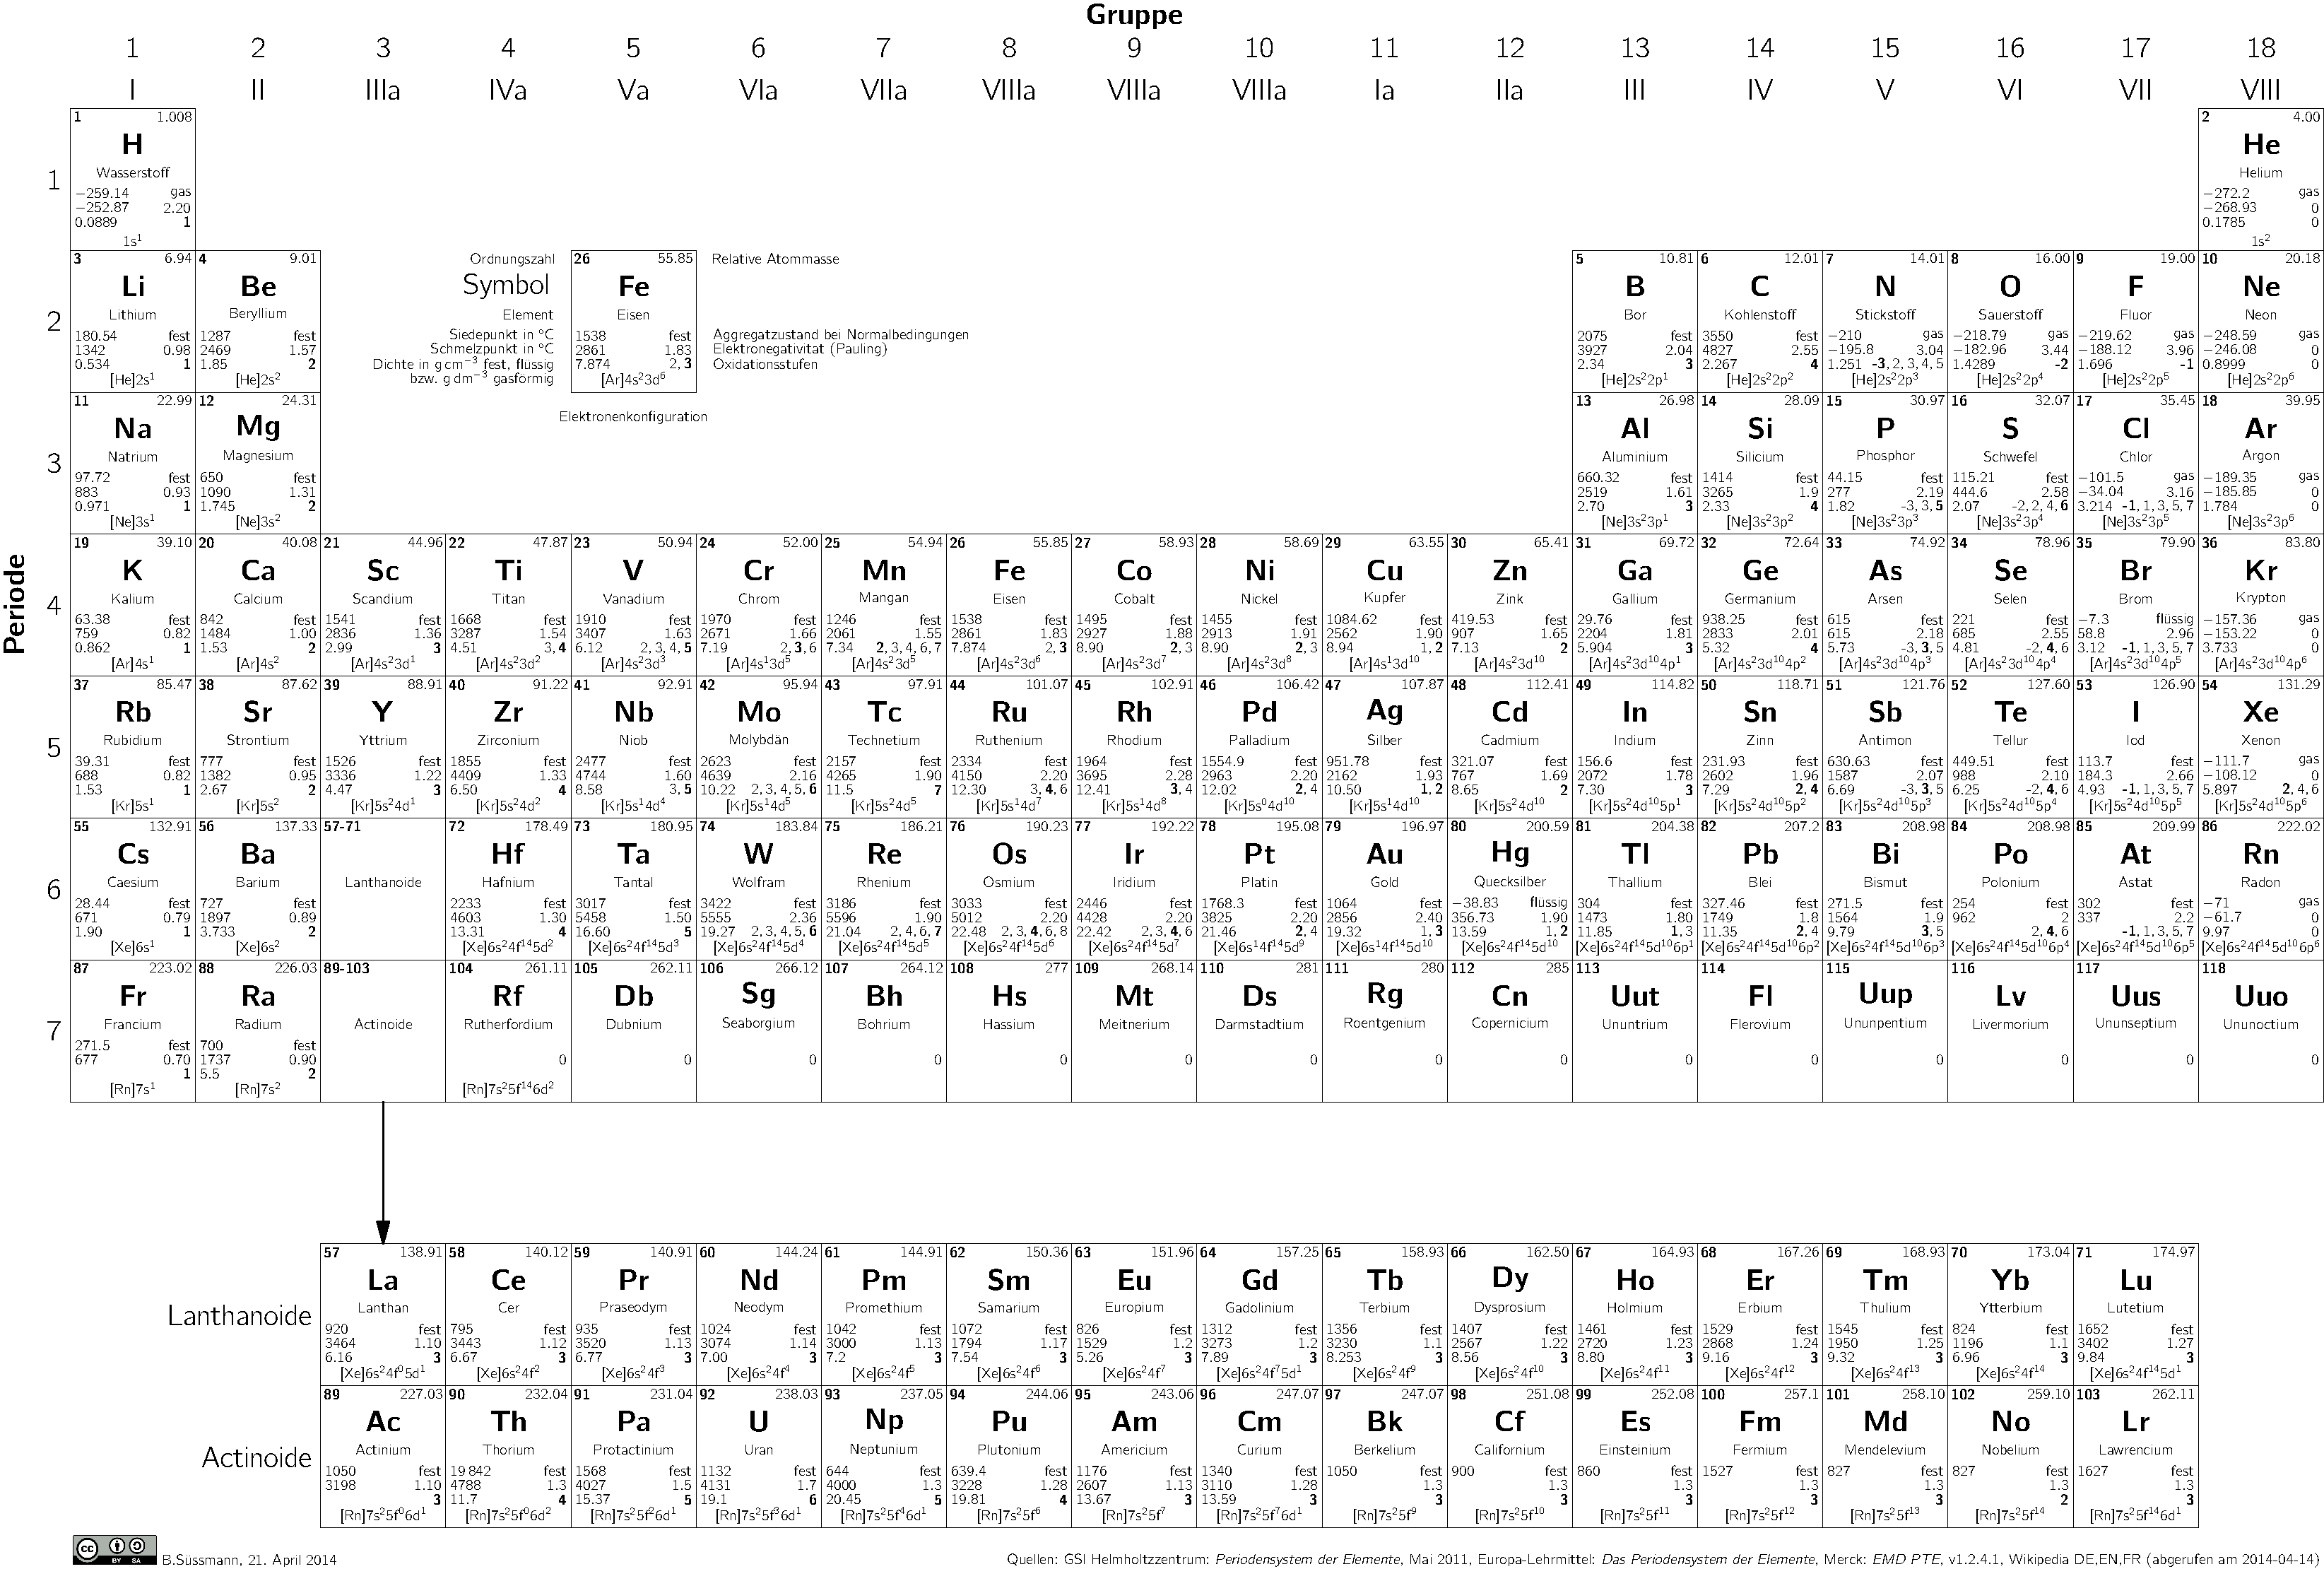
\includegraphics[angle=90,height=.95\textheight]{elemente/periodictable_monochrome}

 
\end{document}
